%% Corrected one-page summary, v3. Build with pdflatex handout.tex.
\documentclass[10pt]{article}
\usepackage[margin=0.5in,letterpaper]{geometry}
\usepackage{graphicx}
\usepackage{booktabs}
\usepackage{xcolor}
\usepackage{hyperref}
\usepackage{titlesec}
\titleformat*{\section}{\small\bfseries}
\titlespacing*{\section}{0pt}{4pt}{1pt}
\pagestyle{empty}
\setlength{\parindent}{0pt}
\setlength{\parskip}{3pt}
\begin{document}
\begin{center}
{\LARGE\textbf{Distribution-Preserving QIM}}\\[2pt]
{\large Histogram detectability and robustness trade-offs}\\[3pt]
{\small Abhishek Sairam Gaduputi, Department of Data Science, NJIT}\\
{\small\texttt{ag2936@njit.edu}}\\
{\small\url{https://github.com/sairam782/Invisible-Watermarking}}
\end{center}

\section*{Corrected result, not a security guarantee}
DP-QIM replaces a mismatched DCT carrier with a sample from the target
quantile cell instead of a lattice point. It reduces some histogram
fingerprints but remains detectable. The previous near-undetectability
claim is withdrawn.

\section*{What the theory actually says}
For ideal continuous equal-mass cells and independent uniform bits,
$P_W=\frac12F+\frac14G_{0,\epsilon}+\frac14G_{1,\epsilon}$, where each
$G_{i,\epsilon}$ is conditioned \emph{within its own safe cell}. Global
conditioning is not equivalent in general. Finite pools, ties and RGB
rounding prevent an exact implementation-level guarantee.
A zero decision boundary is invariant to positive scalar scaling; this is
not a theorem about image blur or resizing. QIM can decode correctly after
large displacements because its label regions repeat periodically.

\begin{center}
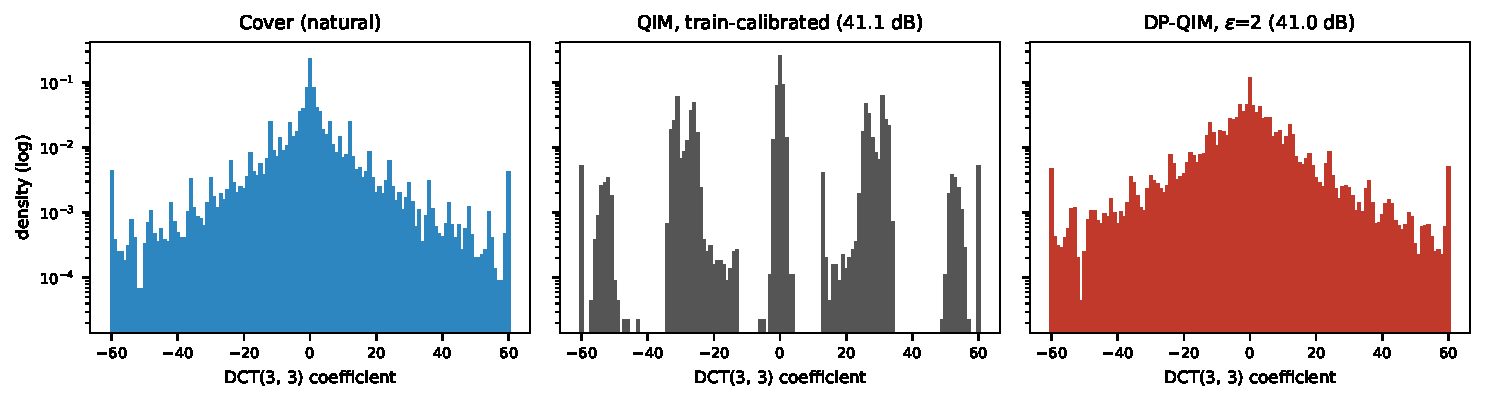
\includegraphics[width=0.85\linewidth]{figures/fig1_histograms_v2.pdf}
\end{center}

\section*{Protocol and corrected measurements}
43 crops from 14 distinct photos; exact source/crop hashes checked.
The \texttt{cat}/\texttt{chelsea} alias is removed. Every detector component
and QIM fidelity calibration uses the same outer training split.
AUC is averaged within folds, not pooled across different classifiers.
Intervals are conditional source bootstraps, not uncertainty over retraining.

\begin{minipage}[t]{0.48\linewidth}
\textbf{Detectability} (0.5 = chance)\\[2pt]
\resizebox{\linewidth}{!}{\begin{tabular}{rcccc}
\toprule
 & \multicolumn{2}{c}{Learned detector} & \multicolumn{2}{c}{Peak statistic} \\
\cmidrule(lr){2-3}\cmidrule(lr){4-5}
Bits (PSNR) & DCT-QIM & DP-QIM & DCT-QIM & DP-QIM \\
\midrule
64 (53.4) & 0.95 [0.91, 1.00] & \textbf{0.65 [0.63, 0.76]} & 0.64 [0.52, 0.77] & \textbf{0.47 [0.41, 0.49]} \\
256 (46.9) & 1.00 [1.00, 1.00] & \textbf{0.84 [0.79, 0.92]} & 0.83 [0.67, 1.00] & \textbf{0.50 [0.39, 0.59]} \\
1024 (41.0) & 1.00 [1.00, 1.00] & \textbf{0.96 [0.91, 1.00]} & 0.97 [0.92, 1.00] & \textbf{0.62 [0.40, 0.80]} \\
\bottomrule
\end{tabular}
}
\end{minipage}\hfill
\begin{minipage}[t]{0.48\linewidth}
\textbf{Robustness} (matched-PSNR difference)\\[2pt]
\resizebox{\linewidth}{!}{\begin{tabular}{lccc}
\toprule
Attack & DP-QIM & $\Delta$ vs.\ DCT-QIM (pp) & 95\% CI \\
\midrule
No attack & 0.999 & -0.1 & [-0.3, +0.0] \\
JPEG $Q{=}90$ & 0.839 & \textbf{-15.2} & [-19.2, -11.8] \\
JPEG $Q{=}70$ & 0.710 & \textbf{-28.4} & [-31.4, -25.3] \\
Gaussian noise $\sigma{=}0.03$ & 0.829 & \textbf{-13.6} & [-16.0, -11.6] \\
Gaussian blur $r{=}1$ & 0.837 & \textbf{+34.6} & [+30.3, +39.6] \\
Downscale $0.5\times$ & 0.831 & \textbf{+34.0} & [+30.5, +37.4] \\
Contrast $\times 0.5$ & 0.967 & \textbf{+19.6} & [+13.5, +30.0] \\
Contrast $\times 0.8$ & 0.975 & -0.3 & [-2.5, +2.0] \\
UnMarker-style ($\tau{=}2$, $j{=}0.5$) & 0.972 & \textbf{-2.8} & [-5.2, -1.0] \\
UnMarker-style ($\tau{=}1.5$, $j{=}1$) & 0.912 & \textbf{-6.9} & [-9.6, -3.9] \\
\bottomrule
\end{tabular}
}
\end{minipage}

\section*{Interpretation and limits}
Learned-detector AUC for DP-QIM rises from 0.65 to 0.84 and 0.96 as
payload increases. At 64 bits, blur/downscale/half-contrast gains are
34.8/33.4/20.8 pp, while JPEG 90/JPEG 70/noise cost 15.8/28.6/14.1 pp.
Histogram-jitter losses are 2.7 to 7.0 pp; this is \emph{not} published UnMarker.
The data were used during development. Independent benchmarks, stronger
detectors and gain-invariant QIM baselines remain necessary. Read the full
paper and \texttt{CORRECTIONS.md}; this summary is not publication validation.
\end{document}
